%%%%%%%%%%%%%%%%%%%%%%%%%%%%%%%%%%%%%%%%%%%%%%%%%%%%%%%%%%%%%%%%%%%%%%%%
% Plantilla TFG/TFM
% Universidad de A Coruña. Facultad de Informática
% Realizado por: Welton Vieira dos Santos
% Modificado: Welton Vieira dos Santos
% Contacto: welton.dossantos@udc.es
%%%%%%%%%%%%%%%%%%%%%%%%%%%%%%%%%%%%%%%%%%%%%%%%%%%%%%%%%%%%%%%%%%%%%%%%


\chapter{Modelo de conocimiento}
\newpage
\section{Fase de identificación}
\subsection{Tareas del formulario OM-3}
La tarea elegida para este modelo conceptual ha sido la tarea 5 del OM-3 (Tabla \ref{tab:IdentificacionOM3}), que corresponde con la \textbf{Gestión de las Operativas Abiertas}.

\begin{table}[H]
  \centering
  \resizebox{18,0cm}{!}{
    \begin{tabular}{|c|c|c|c|c|c|c|}
      \hline
      \multicolumn{3}{|c}{\textbf{Modelo de Organización}} & \multicolumn{4}{|c|}{\textbf{Formulario OM-3: Descomposición de los Procesos}}\\
      \hline \hline
      \textsc{N\textordmasculine} & \textsc{Tarea} & \textsc{Realiza\-da por} & \textsc{¿Dónde?} & \textsc{Recursos de Conocimiento} & \textsc {¿In\-ten\-si\-va en Conocimiento?} & \textsc{Im\-por\-tan\-cia} \\
      \hline
            
      5 & \multicolumn{1}{|p{6.0cm}|}{\centering Gestionar las operativas abiertas} & \multicolumn{1}{|p{6.0cm}|}{\centering Inversor (usuario)} &  \multicolumn{1}{|p{5.0cm}|}{\centering En PC del inversor (usuario)} & \multicolumn{1}{|p{6.0cm}|}{\centering Experiencia en gestionar las operativas de compra y venta de activos al mercado de divisas. Teorías de gestión de capital de inversión} & Sí (elevado) & Máxima \\
      \hline
    \end{tabular}
  }
	\caption{\label{tab:IdentificacionOM3}Tarea elegida para el modelo de conocimiento}
\end{table}

\subsection{Glosario de términos}
\begin{itemize}
	\item \textbf{Activo:} Entidad en la que se prentende especular, que en caso de Forex, hay una variabilidad de 26 pares de divisas, por ejemplo, EURUSD - Euro contra el Dolar.
	\item \textbf{Tendencia Alcista:} es una tendencia del mercado bulsátil donde los precios de los activos financieros llegan a nuevos máximos comparando en un mismo período de análisis. Ejemplo en la imagen de la izquierda de la Figura \ref{fig:EjemploTentendias}.
	\item \textbf{Tendencia Bajista:} es una tendencia del mercado bulsátil donde los precios de los activos financieros llegan a nuevos mínimos comparando en un mismo período de análisis. Ejemplo en la imagen de la derecha de la Figura \ref{fig:EjemploTentendias}.
	\item \textbf{Soporte:} Un soporte es un nivel de precio por debajo del actual, se espera que la fuerza de compra supere a la de venta, por lo que un impulso bajista se verá frenado y por lo tanto el precio repuntará. Normalmente, un soporte corresponde a un mínimo alcanzado anteriormente. Ejemplos en la Figura \ref{fig:SoportesResistencias} se muestra como lineas horizontales de color azul (S1,S2,\dots,SN)
	\item \textbf{Resistencia:} Una resistencia es el concepto opuesto a un soporte. Es un precio por encima del actual, la fuerza de venta superará a la de compra, poniendo fin al impulso alcista, y por lo tanto el precio retrocederá. Ejemplos en la Figura \ref{fig:SoportesResistencias} se muestra como lineas horizontales de color azul (S1,S2,\dots,SN).
	\item \textbf{Stop Loss:} Son límites máximos de pérdida puesto por parte del inversor para frenar una situación de pérdida.
\end{itemize}

\begin{figure}[H]
	\centering
	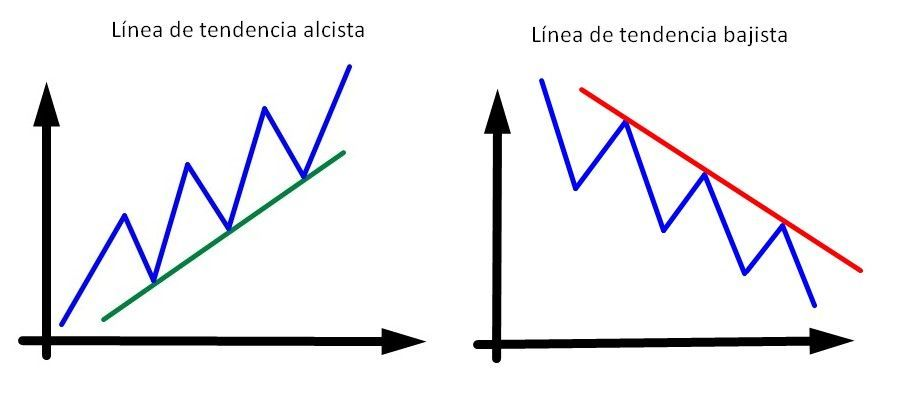
\includegraphics[scale=0.45]{imagenes/EjemploTentendias.png}
	\caption{\label{fig:EjemploTentendias}Ejemplo de tendencias de mercado}
\end{figure}

\begin{figure}[H]
	\centering
	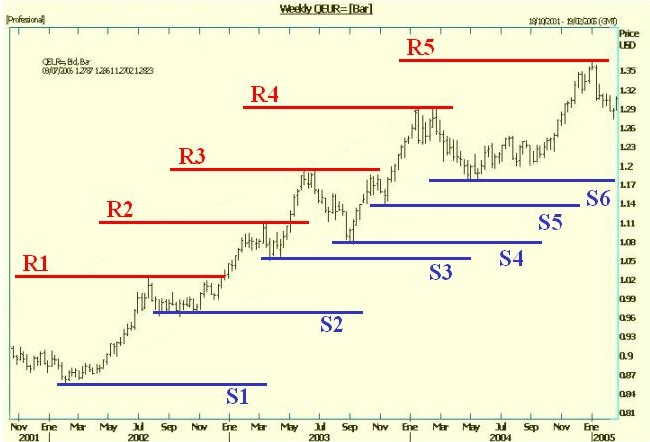
\includegraphics[scale=0.45]{imagenes/SoportesResistencias.png}
	\caption{\label{fig:SoportesResistencias}Soportes y resistencias del Euro/Dólar de 2001 a 2005}
\end{figure}

\subsection{Descripción de escenarios}
\begin{enumerate}
	\item  \textbf{Escenario de reducción de riesgo de una orden de compra (Buy):} En la situación que se muestra en la Figura \ref{fig:Situacion1}, donde el inversor había ejecutado una orden de compra en el precio \textbf{1.18767} y ha estipulado su gestión de riesgo para el precio \textbf{1.18664} y como se observa en el gráfico de la figura comentada anteriormente, el precio esta a favor del inversor y en esa ocasión el inversor tiene que reducir el riesgo inicial de la inversión al precio \textbf{1.19516} como se muestra en la Figura \ref{fig:Situacion12}.	
	\item  \textbf{Escenario de gestión de ganancia en una orden de compra (Buy)}: En la situación que se muestra en la Figura \ref{fig:Situacion2}, donde el inversor había ejecutado una orden de compra en el precio \textbf{1.18767} y ha estipulado su gestión de riesgo para el precio \textbf{1.18664} y como se observa en el gráfico de la figura comentada anteriormente, el precio esta a favor del inversor y el mismo decide cerrar esa operativa a precio del mercado, que en ese caso es de \textbf{1.19665}.	
\end{enumerate}
\begin{figure}[H]
    \centering
    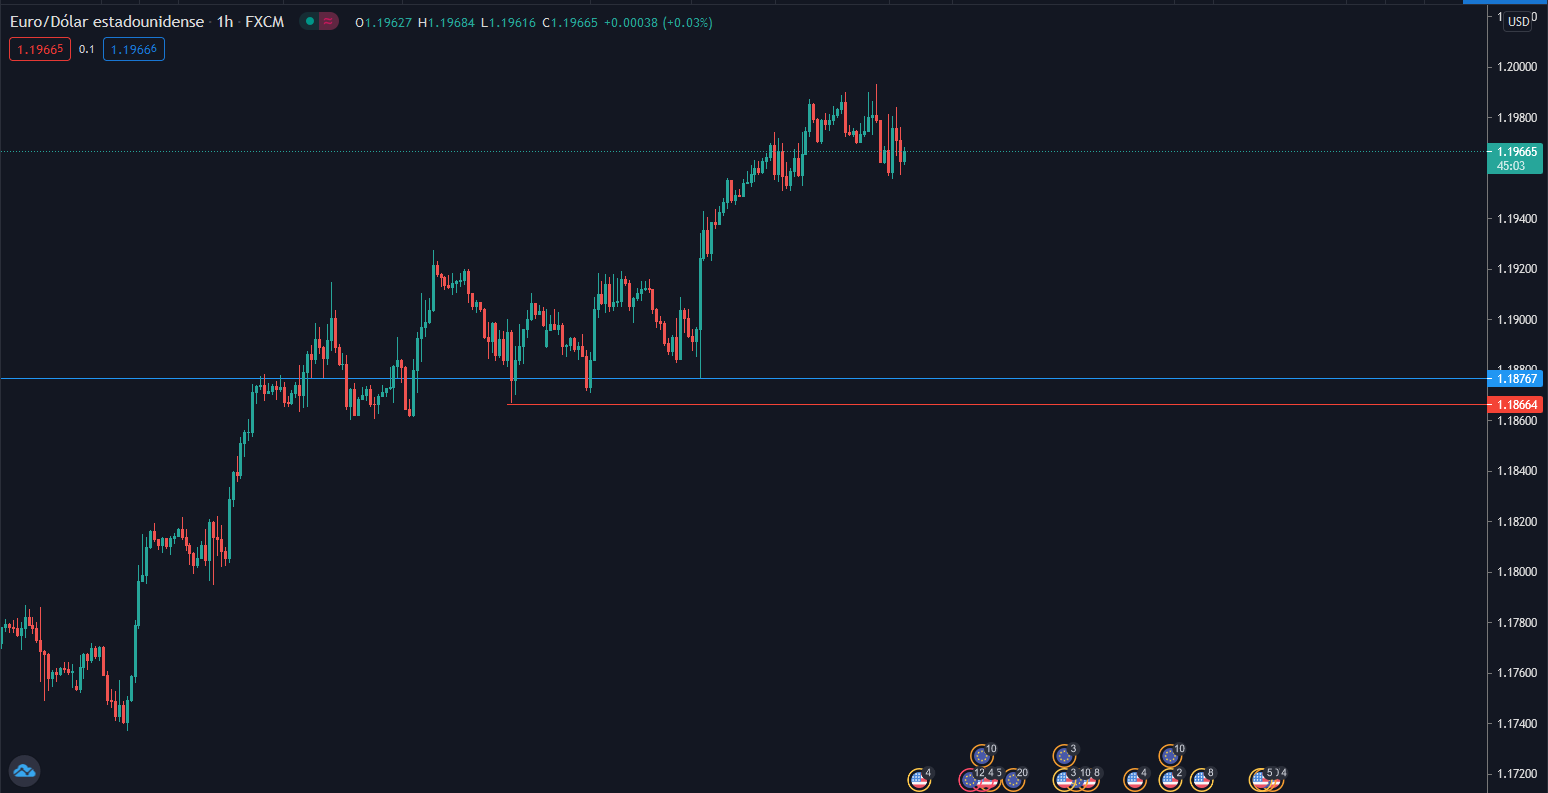
\includegraphics[scale=0.30]{imagenes/Situacion1.png}
    \caption{\label{fig:Situacion1}Ejemplo de una situación donde el inversor tiene que ajustar el riesgo de la operativa y seguir dentro del mercado}
  \end{figure}
\begin{figure}[H]
  \centering
  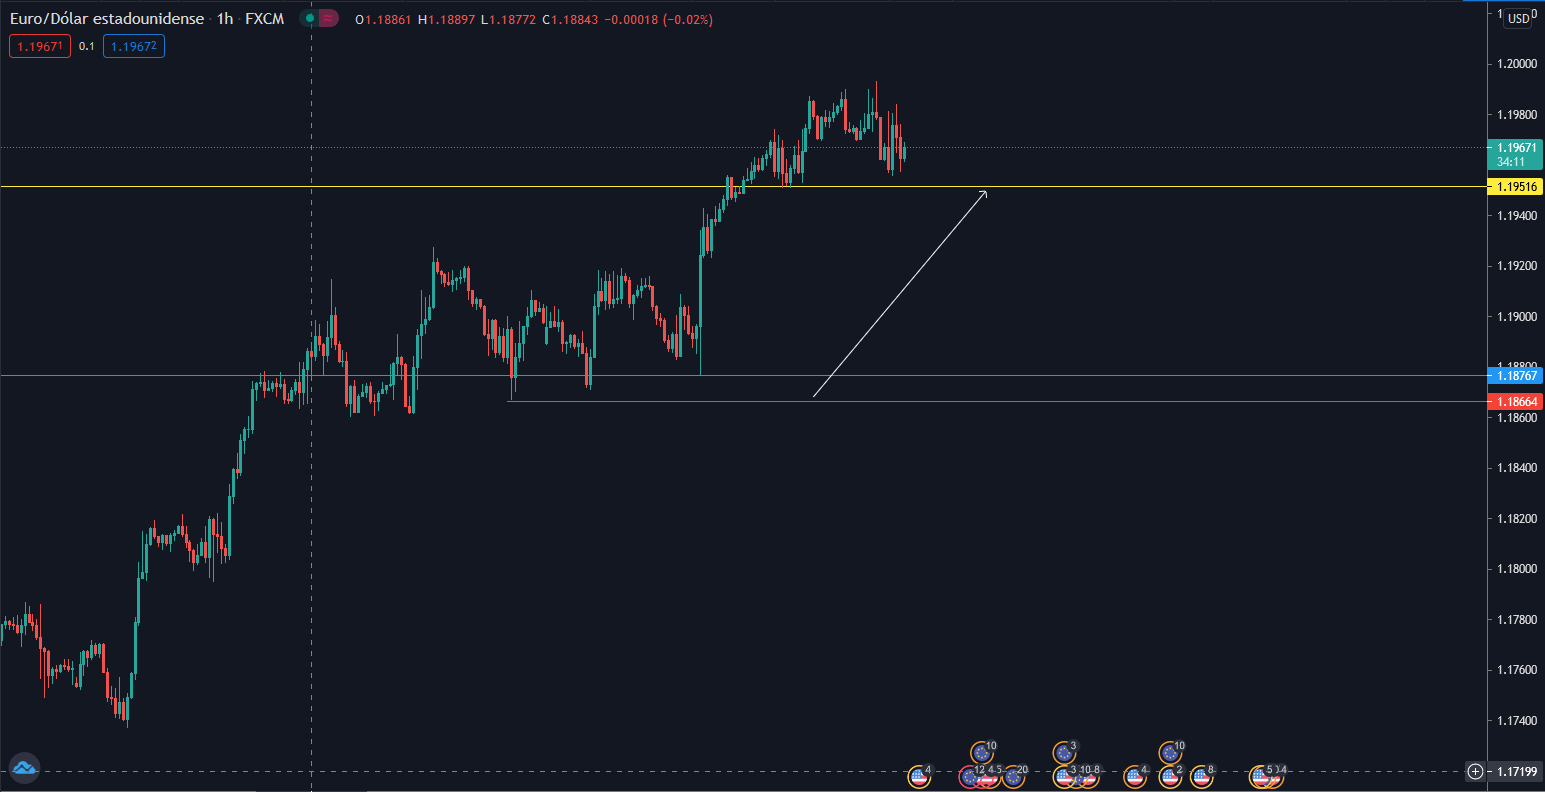
\includegraphics[scale=0.30]{imagenes/Situacion12.png}
  \caption{\label{fig:Situacion12}Ejemplo donde el inversor modifica el nivel de riesgo inicial y mantiene la orden de compra en el mercado}
\end{figure}
\begin{figure}[H]
  \centering
  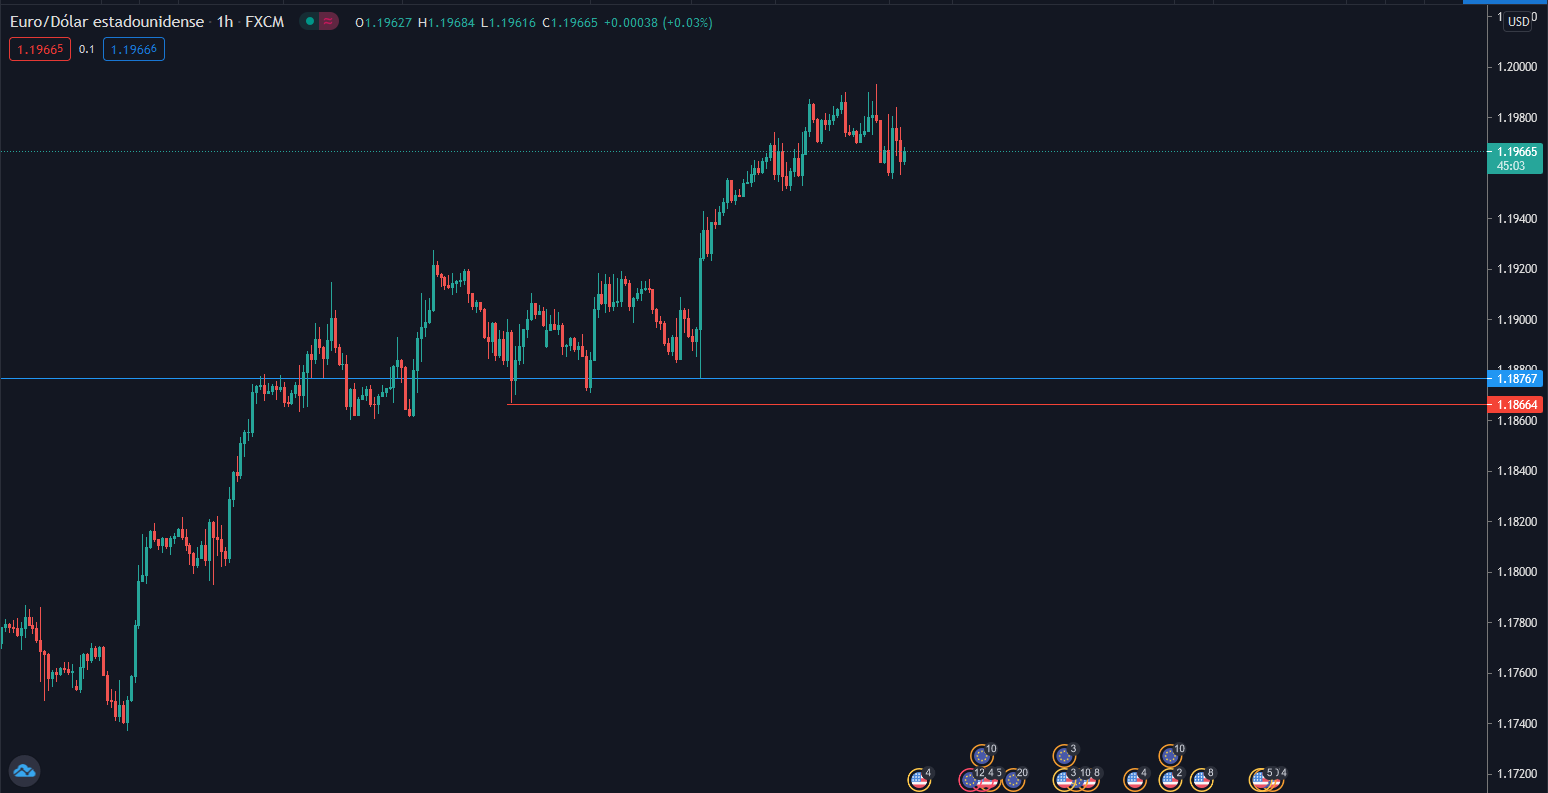
\includegraphics[scale=0.30]{imagenes/Situacion1.png}
  \caption{\label{fig:Situacion2}Ejemplo donde el inversor decide cerrar la orden de compra a precio de mercado}
\end{figure}

\section{Fase de especificación}
\subsection{Justificación de la selección de la metodología}
Para este proyecto hemos decidido utilizar la metodología ``middle-out'' con la selección de la plantilla de diagnóstico, ya que esa plantilla nos permite tomar varias decisiones un proyecto anterior con la misma metodología ``middle-out'', puesto que, además ser muy utilizada en nuestro caso sigue adaptandose perfectamente. 

\subsection{Plantilla anotada}

La plantilla que mas se adapta a nuestro problema es la de diagnóstico, como se muestra en la Figura \ref{fig:PlantillaEjemplo}. Con una pequeña modificación que se muestras en la Figuras \ref{fig:CasoMoverRiesgo} y \ref{fig:CasoCerrarOrden}.

\begin{figure}[H]
  \centering
  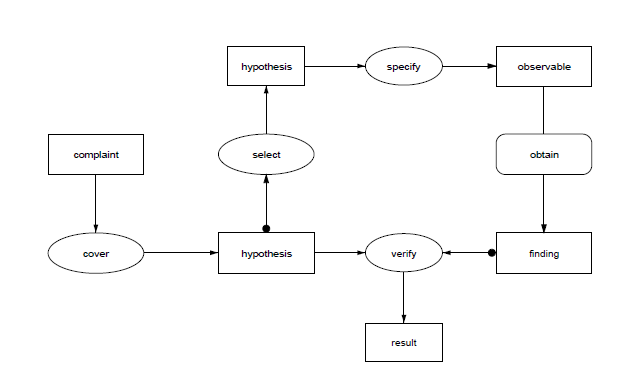
\includegraphics[scale=0.90]{imagenes/PlantillaEjemplo.png}
  \caption{\label{fig:PlantillaEjemplo}Ejemplo de la plantilla elegida}
\end{figure}

\begin{figure}[H]
  \centering
  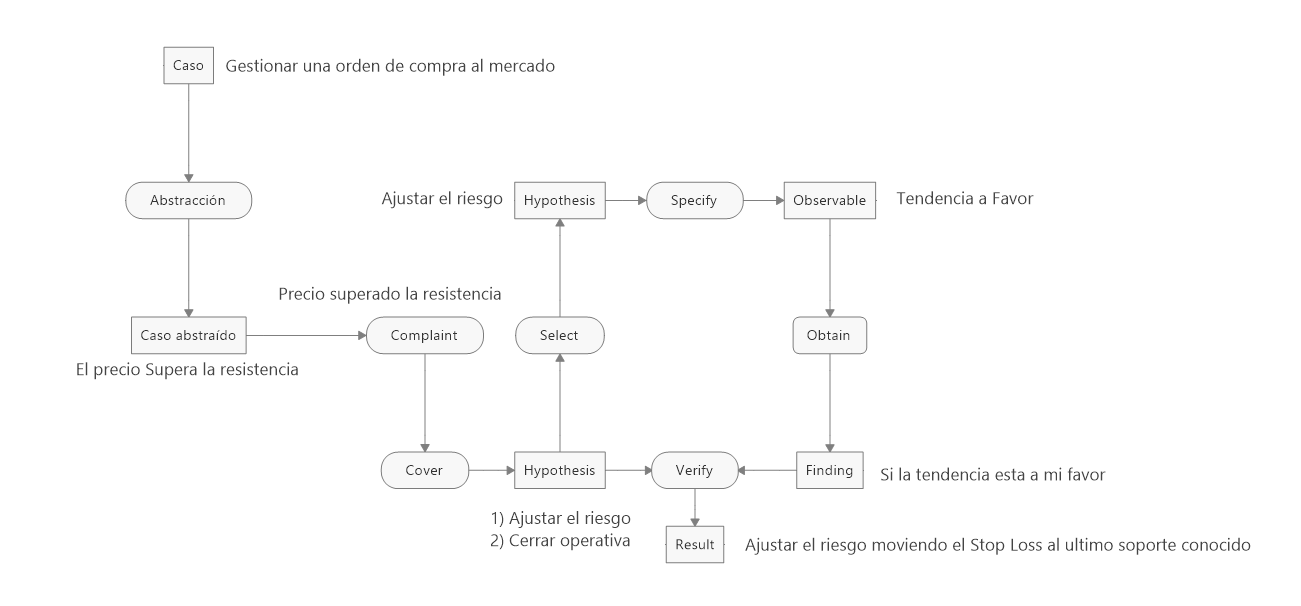
\includegraphics[scale=0.50]{imagenes/CasoMoverRiesgo.png}
  \caption{\label{fig:CasoMoverRiesgo}Ejemplo de la plantilla caso de ajustar riesgo}
\end{figure}

\begin{figure}[H]
  \centering
  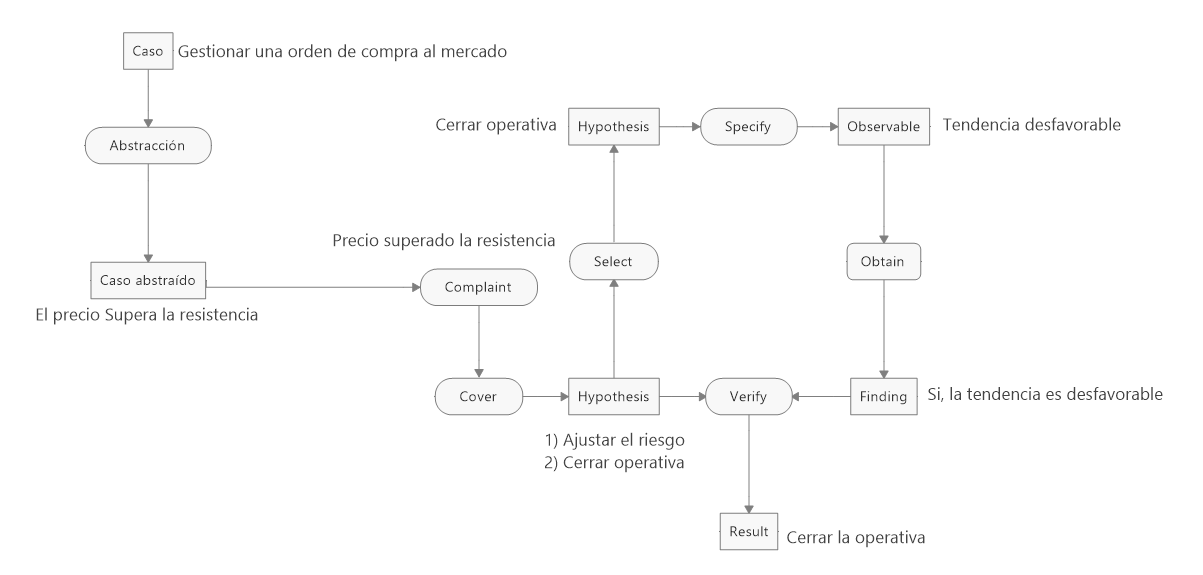
\includegraphics[scale=0.50]{imagenes/CasoCerrarOrden.png}
  \caption{\label{fig:CasoCerrarOrden}Ejemplo de la plantilla con el caso cerrar orden}
\end{figure}

\subsection{Esquema inicial del dominio}

\begin{figure}[H]
  \centering
  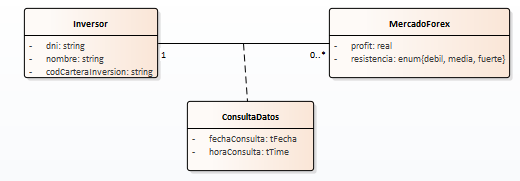
\includegraphics[scale=0.70]{imagenes/DominioInicial.png}
  \caption{\label{fig:DominioInicial}Dominio inicial}
\end{figure}

\subsection{Estructura inferencial}
\subsubsection{Plantilla}
\subsubsection{Mapeado}
Relacción entre los roles de las inferencias de la plantilla con los conceptos de nuestro problema.
\begin{itemize}
  \item Cover:  
  \begin{figure}[H]
    \centering
    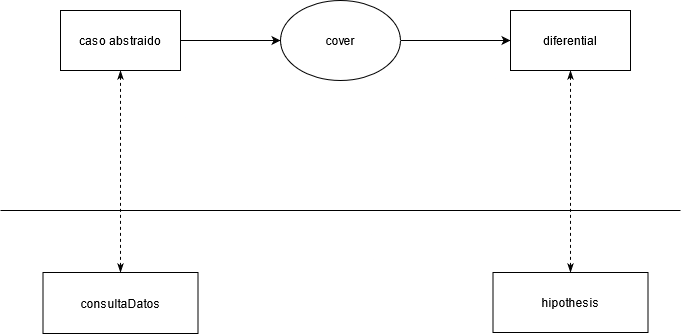
\includegraphics[scale=0.50]{imagenes/Cover.png}
    \caption{\label{fig:Cover}Ejemplo del mapeo de Cover}
  \end{figure}
  \item Select: 
  \begin{figure}[H]
    \centering
    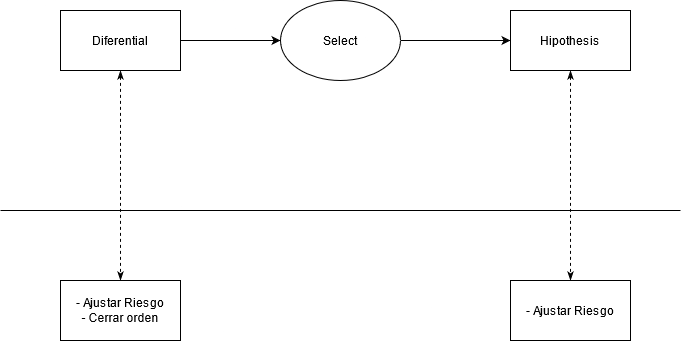
\includegraphics[scale=0.50]{imagenes/Select.png}
    \caption{\label{fig:Select}Ejemplo del mapeo de Select}
  \end{figure}
  \newpage
  \item Specify: 
  \begin{figure}[H]
    \centering
    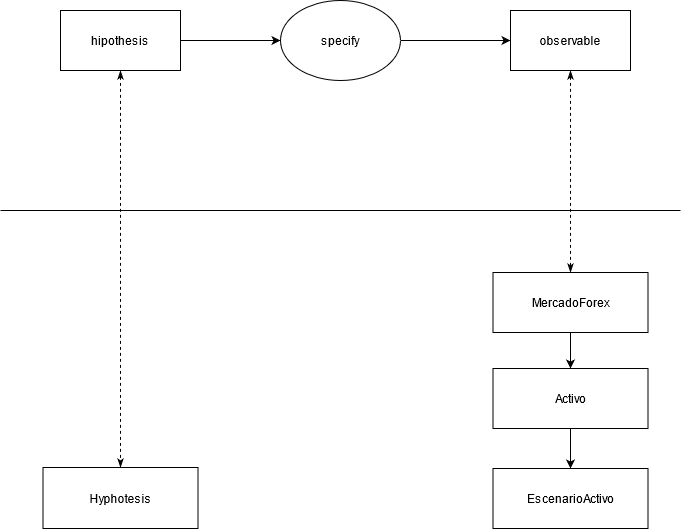
\includegraphics[scale=0.50]{imagenes/Specify.png}
    \caption{\label{fig:Specify}Ejemplo del mapeo de Specify}
  \end{figure}
  \item Obtain:  
  \begin{figure}[H]
    \centering
    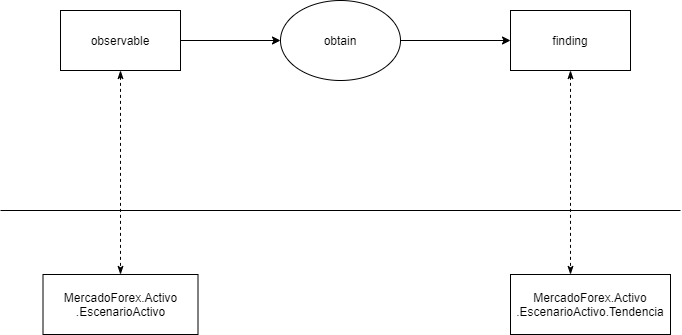
\includegraphics[scale=0.50]{imagenes/Obtain.png}
    \caption{\label{fig:Obtain}Ejemplo del mapeo de Obtain}
  \end{figure}
  \newpage
  \item Verify:  
  \begin{figure}[H]
    \centering
    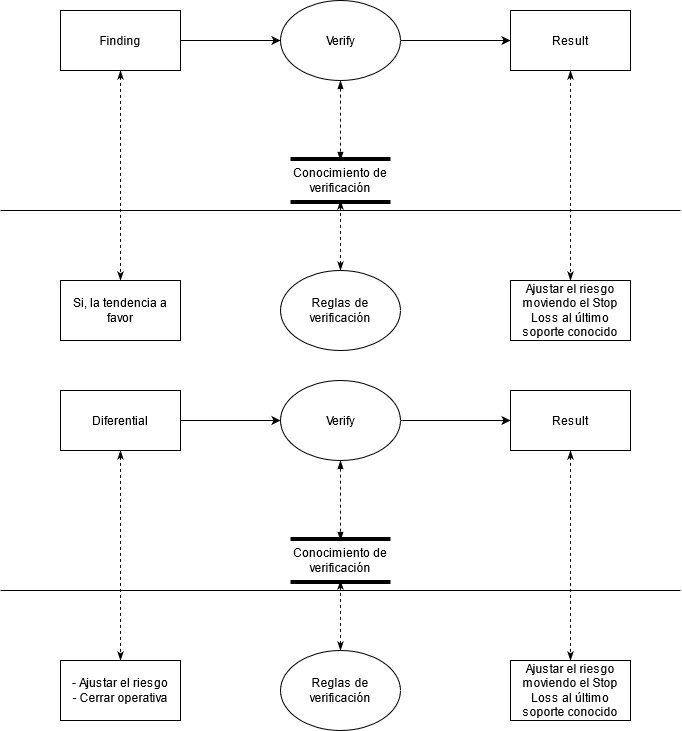
\includegraphics[scale=0.50]{imagenes/Verify.png}
    \caption{\label{fig:Verify}Ejemplo del mapeo de Verify}
  \end{figure}
\end{itemize}

\section{Especificación y método de la tarea}